\documentclass[11pt]{article}

\usepackage[T1]{fontenc}
\usepackage[utf8]{inputenc}
\usepackage{lmodern}
\usepackage{amsmath,amssymb,amsthm,mathtools}
\usepackage{microtype}
\usepackage{booktabs}
\usepackage{enumitem}
\usepackage{tabularx}
\usepackage{needspace}
\usepackage{array}
\usepackage[margin=1in,top=0.9in,bottom=1in]{geometry}
\usepackage{fancyhdr}
\usepackage{lastpage}
\usepackage{tikz}
\usepackage[hidelinks]{hyperref}

\pagestyle{fancy}
\fancyhf{}
\lhead{\small BIO 2970 --- Selection Practice Exam S1}
\rhead{\small Name: \underline{\hspace{5cm}}}
\cfoot{\small\thepage\ of \pageref*{LastPage}}
\renewcommand{\headrulewidth}{0.4pt}
\setlength{\headheight}{14pt}

% answer text, for KEY documents only
\newcommand{\keyans}[1]{\par\medskip\noindent\textit{Answer.}\ #1\par\medskip}
\newcommand{\work}[1]{\par\vspace{#1}}
\newcommand{\opt}[1]{\makebox[1.9em][l]{(#1)}}
\newcolumntype{Y}{>{\raggedright\arraybackslash}X}
\setlist[enumerate,1]{leftmargin=2em,labelsep=0.6em}
\hyphenpenalty=1000
\relpenalty=10000
\binoppenalty=10000
\begin{document}

\begin{center}
  {\LARGE\bfseries Natural Selection --- Practice Exam S1}\\[5pt]
  {\large Level 1 \quad\textbullet\quad Quiz difficulty}\\[6pt]
  BIO 2970 \quad\textbullet\quad Fitness and Selection, Lectures 23 and 24 \quad\textbullet\quad Fall 2026\\[3pt]
  \rule{\textwidth}{0.8pt}\\[3pt]
  {\small Every kind of question last year's quiz asked, plus the definitions and model choices underneath them.\\[2pt] 24 multiple-choice questions of equal weight. Choose the single best answer and mark it on the answer sheet on the second-to-last page. Calculator allowed. Give three decimals unless a question says otherwise.}
\end{center}
\vspace{0.4em}

\begin{enumerate}[label=\textbf{\arabic*.}, leftmargin=2em, itemsep=1.4em]
\needspace{9\baselineskip}
\item Viability is 0.4, 0.4 and 0.2 for AA, Aa and aa. Lifetime fecundity is 5, 5 and 8. What is the absolute fitness \(w\) of aa?
\par\smallskip\noindent\begin{tabularx}{\linewidth}{@{}YYYY@{}}
\makebox[1.9em][l]{(A)}8.2 & \makebox[1.9em][l]{(B)}0.2 & \makebox[1.9em][l]{(C)}1.6 & \makebox[1.9em][l]{(D)}2.0 \\
\end{tabularx}
\work{1.6cm}
\needspace{9\baselineskip}
\item Same genotypes. What are the relative fitness \(W\) and the selection coefficient \(s\) of aa?
\par\smallskip\noindent\begin{tabularx}{\linewidth}{@{}YY@{}}
\makebox[1.9em][l]{(A)}\(W\) = 0.8, \(s\) = 0.2 & \makebox[1.9em][l]{(B)}\(W\) = 0.2, \(s\) = 0.8 \\[3pt]
\makebox[1.9em][l]{(C)}\(W\) = 1.6, \(s\) = \(-\)0.6 & \makebox[1.9em][l]{(D)}\(W\) = 0.8, \(s\) = 0.8 \\
\end{tabularx}
\needspace{9\baselineskip}
\item A population has 110 AA, 50 Aa and 40 aa. Calculate \(q^2\), the way last year's quiz asked.
\par\smallskip\noindent\begin{tabularx}{\linewidth}{@{}YYYY@{}}
\makebox[1.9em][l]{(A)}0.200 & \makebox[1.9em][l]{(B)}0.325 & \makebox[1.9em][l]{(C)}0.447 & \makebox[1.9em][l]{(D)}0.106 \\
\end{tabularx}
\work{1.6cm}
\needspace{9\baselineskip}
\item Same population. Relative fitnesses are 1, 0.8 and 0.5. Calculate \(\overline{W}\) using \(p^2\), \(2pq\) and \(q^2\).
\par\smallskip\noindent\begin{tabularx}{\linewidth}{@{}YYYY@{}}
\makebox[1.9em][l]{(A)}0.85 & \makebox[1.9em][l]{(B)}0.86 & \makebox[1.9em][l]{(C)}0.77 & \makebox[1.9em][l]{(D)}1.00 \\
\end{tabularx}
\work{1.6cm}
\needspace{9\baselineskip}
\item Lizards of medium body size survive best. Small ones lose fights and large ones are easier for hawks to see. Which type of selection is this?
\par\smallskip\noindent\begin{tabularx}{\linewidth}{@{}YYYY@{}}
\makebox[1.9em][l]{(A)}Directional & \makebox[1.9em][l]{(B)}Stabilizing & \makebox[1.9em][l]{(C)}Disruptive & \makebox[1.9em][l]{(D)}Balancing \\
\end{tabularx}
\needspace{9\baselineskip}
\item In polluted forests the dark peppered moth allele rose from rare to over 90 percent. At the level of the allele, which type of selection is this?
\par\smallskip\noindent\begin{tabularx}{\linewidth}{@{}YY@{}}
\makebox[1.9em][l]{(A)}Negative (purifying) & \makebox[1.9em][l]{(B)}Balancing \\[3pt]
\makebox[1.9em][l]{(C)}Stabilizing & \makebox[1.9em][l]{(D)}Positive \\
\end{tabularx}
\needspace{9\baselineskip}
\item Finches with very small beaks eat soft seeds and finches with very large beaks crack hard seeds. Birds in between starve. Which type of selection is this?
\par\smallskip\noindent\begin{tabularx}{\linewidth}{@{}YYYY@{}}
\makebox[1.9em][l]{(A)}Disruptive & \makebox[1.9em][l]{(B)}Stabilizing & \makebox[1.9em][l]{(C)}Directional & \makebox[1.9em][l]{(D)}Balancing \\
\end{tabularx}
\needspace{9\baselineskip}
\item A new frameshift mutation in an essential gene keeps appearing and keeps being removed because carriers rarely reproduce. Which type of selection removes it?
\par\smallskip\noindent\begin{tabularx}{\linewidth}{@{}YY@{}}
\makebox[1.9em][l]{(A)}Positive & \makebox[1.9em][l]{(B)}Balancing \\[3pt]
\makebox[1.9em][l]{(C)}Negative (purifying) & \makebox[1.9em][l]{(D)}Disruptive \\
\end{tabularx}
\needspace{9\baselineskip}
\item In cattle, hornless (H) is completely dominant to horned (h). Horned animals are injured more often and survive less. Which selection model is best to use?
\par\smallskip
\begin{enumerate}[label={}, leftmargin=2.4em, labelwidth=0pt, itemsep=2pt, topsep=0pt]
\item \hspace*{-2.4em}\makebox[2.4em][l]{(A)}Complete dominance with selection against the dominant
\item \hspace*{-2.4em}\makebox[2.4em][l]{(B)}Heterozygote advantage
\item \hspace*{-2.4em}\makebox[2.4em][l]{(C)}No special model applies
\item \hspace*{-2.4em}\makebox[2.4em][l]{(D)}Complete dominance with selection against the recessive
\end{enumerate}
\needspace{9\baselineskip}
\item Same cattle. Assign the symbols for the selection model equation.
\par\smallskip\noindent\begin{tabularx}{\linewidth}{@{}YY@{}}
\makebox[1.9em][l]{(A)}H = \(q\) and h = \(p\) & \makebox[1.9em][l]{(B)}Either way gives the same \(\Delta q\) \\[3pt]
\makebox[1.9em][l]{(C)}H = \(p\) and h = \(q\) & \makebox[1.9em][l]{(D)}H = \(p\) and h = \(p\) \\
\end{tabularx}
\needspace{9\baselineskip}
\item Same cattle. The selection coefficient for horned animals is 0.3. What is their relative fitness?
\par\smallskip\noindent\begin{tabularx}{\linewidth}{@{}YYYY@{}}
\makebox[1.9em][l]{(A)}0.3 & \makebox[1.9em][l]{(B)}0.7 & \makebox[1.9em][l]{(C)}1.3 & \makebox[1.9em][l]{(D)}0.0 \\
\end{tabularx}
\work{1.6cm}
\needspace{9\baselineskip}
\item Same cattle. Is it more appropriate to calculate \(\Delta q\) or \(\hat{q}\)?
\par\smallskip\noindent\begin{tabularx}{\linewidth}{@{}YY@{}}
\makebox[1.9em][l]{(A)}\(\Delta q\) & \makebox[1.9em][l]{(B)}\(\hat{q}\) \\[3pt]
\makebox[1.9em][l]{(C)}Both are equally appropriate & \makebox[1.9em][l]{(D)}Neither, because h is recessive \\
\end{tabularx}
\needspace{9\baselineskip}
\item Three genotypes have fecundities 2, 3 and 4 for AA, Aa and aa, frequencies 0.5, 0.4 and 0.1, and equal survival. What is the frequency of a after selection?
\par\smallskip\noindent\begin{tabularx}{\linewidth}{@{}YYYY@{}}
\makebox[1.9em][l]{(A)}0.300 & \makebox[1.9em][l]{(B)}0.615 & \makebox[1.9em][l]{(C)}0.385 & \makebox[1.9em][l]{(D)}0.154 \\
\end{tabularx}
\work{1.6cm}
\needspace{9\baselineskip}
\item In \(\Delta q\) = (\(q\)/\(\overline{W}\))\(\cdot \alpha_{a}\), which part determines whether the allele increases or decreases?
\par\smallskip
\begin{enumerate}[label={}, leftmargin=2.4em, labelwidth=0pt, itemsep=2pt, topsep=0pt]
\item \hspace*{-2.4em}\makebox[2.4em][l]{(A)}The average excess \(\alpha_{a}\)
\item \hspace*{-2.4em}\makebox[2.4em][l]{(B)}Mean fitness \(\overline{W}\)
\item \hspace*{-2.4em}\makebox[2.4em][l]{(C)}The allele frequency \(q\)
\item \hspace*{-2.4em}\makebox[2.4em][l]{(D)}The Hardy-Weinberg genotype frequencies
\end{enumerate}
\needspace{9\baselineskip}
\item Hardy-Weinberg, \(q\) = 0.3, relative fitnesses 1, 0.8 and 0.6 for AA, Aa and aa. What is the average excess of a?
\par\smallskip\noindent\begin{tabularx}{\linewidth}{@{}YYYY@{}}
\makebox[1.9em][l]{(A)}+0.14 & \makebox[1.9em][l]{(B)}\(-\)0.32 & \makebox[1.9em][l]{(C)}0.74 & \makebox[1.9em][l]{(D)}\(-\)0.14 \\
\end{tabularx}
\work{1.6cm}
\needspace{9\baselineskip}
\item Wolves have absolute fitnesses 3, 5 and 4 for B1B1, B1B2 and B2B2. What is the equilibrium frequency of B2?
\par\smallskip\noindent\begin{tabularx}{\linewidth}{@{}YYYY@{}}
\makebox[1.9em][l]{(A)}0.333 & \makebox[1.9em][l]{(B)}0.667 & \makebox[1.9em][l]{(C)}0.500 & \makebox[1.9em][l]{(D)}0.800 \\
\end{tabularx}
\work{1.6cm}
\needspace{9\baselineskip}
\item Why is the equilibrium under heterozygote advantage stable?
\par\smallskip
\begin{enumerate}[label={}, leftmargin=2.4em, labelwidth=0pt, itemsep=2pt, topsep=0pt]
\item \hspace*{-2.4em}\makebox[2.4em][l]{(A)}The heterozygotes cannot reproduce
\item \hspace*{-2.4em}\makebox[2.4em][l]{(B)}Whichever allele is rare sits mostly in fit heterozygotes, so it is favored and rises back
\item \hspace*{-2.4em}\makebox[2.4em][l]{(C)}Mutation keeps restoring both alleles
\item \hspace*{-2.4em}\makebox[2.4em][l]{(D)}Drift pushes frequencies toward 0.5
\end{enumerate}
\needspace{9\baselineskip}
\item In a region with intense malaria, which genotype has the highest fitness?
\par\smallskip\noindent\begin{tabularx}{\linewidth}{@{}YY@{}}
\makebox[1.9em][l]{(A)}HbA/HbA & \makebox[1.9em][l]{(B)}HbS/HbS \\[3pt]
\makebox[1.9em][l]{(C)}All three are equal & \makebox[1.9em][l]{(D)}HbA/HbS \\
\end{tabularx}
\needspace{9\baselineskip}
\item Which three things must be true for selection to change a trait across generations?
\par\smallskip
\begin{enumerate}[label={}, leftmargin=2.4em, labelwidth=0pt, itemsep=2pt, topsep=0pt]
\item \hspace*{-2.4em}\makebox[2.4em][l]{(A)}It varies, it is heritable, and it affects fitness
\item \hspace*{-2.4em}\makebox[2.4em][l]{(B)}It is dominant, common and visible
\item \hspace*{-2.4em}\makebox[2.4em][l]{(C)}It is new, beneficial and fixed
\item \hspace*{-2.4em}\makebox[2.4em][l]{(D)}It varies, it is recessive, and it is rare
\end{enumerate}
\needspace{9\baselineskip}
\item In the Deme lab, many populations start at 0.5 and run for 50 generations. Histogram X is tightly bunched near zero change and histogram Y is spread widely. Which is true?
\par\smallskip
\begin{enumerate}[label={}, leftmargin=2.4em, labelwidth=0pt, itemsep=2pt, topsep=0pt]
\item \hspace*{-2.4em}\makebox[2.4em][l]{(A)}X came from smaller populations than Y
\item \hspace*{-2.4em}\makebox[2.4em][l]{(B)}X experienced selection and Y did not
\item \hspace*{-2.4em}\makebox[2.4em][l]{(C)}X came from larger populations than Y
\item \hspace*{-2.4em}\makebox[2.4em][l]{(D)}Y ran for fewer generations
\end{enumerate}
\needspace{9\baselineskip}
\item Why is the heterozygote term multiplied by \(\tfrac{1}{2}\) in general equation \#1?
\par\smallskip
\begin{enumerate}[label={}, leftmargin=2.4em, labelwidth=0pt, itemsep=2pt, topsep=0pt]
\item \hspace*{-2.4em}\makebox[2.4em][l]{(A)}Heterozygotes have half the fitness
\item \hspace*{-2.4em}\makebox[2.4em][l]{(B)}Heterozygotes are half as common
\item \hspace*{-2.4em}\makebox[2.4em][l]{(C)}It corrects for Hardy-Weinberg
\item \hspace*{-2.4em}\makebox[2.4em][l]{(D)}Only one of a heterozygote's two allele copies is the allele being tracked
\end{enumerate}
\needspace{9\baselineskip}
\item Dominant allele B makes beetles conspicuous. BB and Bb have relative fitness 0.6, and bb has 1. The frequency of B is 0.2, Hardy-Weinberg. What is \(\Delta q\) for B?
\par\smallskip\noindent\begin{tabularx}{\linewidth}{@{}YYYY@{}}
\makebox[1.9em][l]{(A)}\(-\)0.013 & \makebox[1.9em][l]{(B)}\(-\)0.051 & \makebox[1.9em][l]{(C)}\(-\)0.060 & \makebox[1.9em][l]{(D)}\(-\)0.021 \\
\end{tabularx}
\work{1.6cm}
\needspace{9\baselineskip}
\item Every genotype's fitness is multiplied by 10. What happens to \(\Delta q\)?
\par\smallskip
\begin{enumerate}[label={}, leftmargin=2.4em, labelwidth=0pt, itemsep=2pt, topsep=0pt]
\item \hspace*{-2.4em}\makebox[2.4em][l]{(A)}It becomes 10 times larger
\item \hspace*{-2.4em}\makebox[2.4em][l]{(B)}Nothing, because \(\overline{W}\) is multiplied by 10 too and the factor cancels
\item \hspace*{-2.4em}\makebox[2.4em][l]{(C)}It becomes 10 times smaller
\item \hspace*{-2.4em}\makebox[2.4em][l]{(D)}It flips sign
\end{enumerate}
\needspace{9\baselineskip}
\item Heterozygotes have the lowest fitness and both homozygotes are fitter. What happens over many generations?
\par\smallskip
\begin{enumerate}[label={}, leftmargin=2.4em, labelwidth=0pt, itemsep=2pt, topsep=0pt]
\item \hspace*{-2.4em}\makebox[2.4em][l]{(A)}An unstable equilibrium, so one allele goes to fixation
\item \hspace*{-2.4em}\makebox[2.4em][l]{(B)}Both alleles are kept at \(\hat{q}\)
\item \hspace*{-2.4em}\makebox[2.4em][l]{(C)}Both alleles are lost
\item \hspace*{-2.4em}\makebox[2.4em][l]{(D)}Nothing changes
\end{enumerate}
\end{enumerate}

\newpage
\begin{center}
  {\Large\bfseries Answer Sheet}\\[3pt]
  {\small\itshape Fill in one circle per question.}\\[2pt]
  \rule{\textwidth}{0.4pt}
\end{center}
\vspace{1.2em}
\noindent\begin{minipage}[t]{0.32\textwidth}\centering
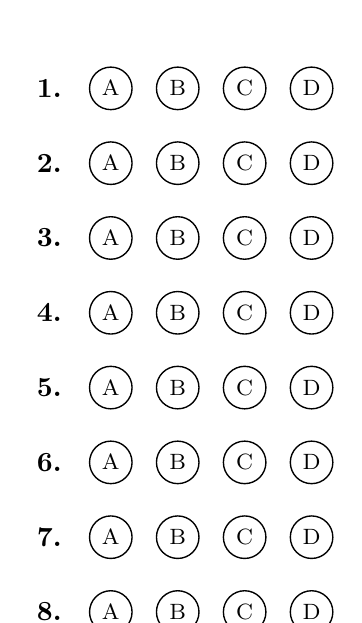
\begin{tikzpicture}[x=1cm,y=1cm]
\node[anchor=east] at (0.55,0.00) {\textbf{1.}};
\draw[line width=0.5pt] (1.05,0.00) circle (0.27);
\node at (1.05,0.00) {\footnotesize A};
\draw[line width=0.5pt] (1.90,0.00) circle (0.27);
\node at (1.90,0.00) {\footnotesize B};
\draw[line width=0.5pt] (2.75,0.00) circle (0.27);
\node at (2.75,0.00) {\footnotesize C};
\draw[line width=0.5pt] (3.60,0.00) circle (0.27);
\node at (3.60,0.00) {\footnotesize D};
\node[anchor=east] at (0.55,-0.95) {\textbf{2.}};
\draw[line width=0.5pt] (1.05,-0.95) circle (0.27);
\node at (1.05,-0.95) {\footnotesize A};
\draw[line width=0.5pt] (1.90,-0.95) circle (0.27);
\node at (1.90,-0.95) {\footnotesize B};
\draw[line width=0.5pt] (2.75,-0.95) circle (0.27);
\node at (2.75,-0.95) {\footnotesize C};
\draw[line width=0.5pt] (3.60,-0.95) circle (0.27);
\node at (3.60,-0.95) {\footnotesize D};
\node[anchor=east] at (0.55,-1.90) {\textbf{3.}};
\draw[line width=0.5pt] (1.05,-1.90) circle (0.27);
\node at (1.05,-1.90) {\footnotesize A};
\draw[line width=0.5pt] (1.90,-1.90) circle (0.27);
\node at (1.90,-1.90) {\footnotesize B};
\draw[line width=0.5pt] (2.75,-1.90) circle (0.27);
\node at (2.75,-1.90) {\footnotesize C};
\draw[line width=0.5pt] (3.60,-1.90) circle (0.27);
\node at (3.60,-1.90) {\footnotesize D};
\node[anchor=east] at (0.55,-2.85) {\textbf{4.}};
\draw[line width=0.5pt] (1.05,-2.85) circle (0.27);
\node at (1.05,-2.85) {\footnotesize A};
\draw[line width=0.5pt] (1.90,-2.85) circle (0.27);
\node at (1.90,-2.85) {\footnotesize B};
\draw[line width=0.5pt] (2.75,-2.85) circle (0.27);
\node at (2.75,-2.85) {\footnotesize C};
\draw[line width=0.5pt] (3.60,-2.85) circle (0.27);
\node at (3.60,-2.85) {\footnotesize D};
\node[anchor=east] at (0.55,-3.80) {\textbf{5.}};
\draw[line width=0.5pt] (1.05,-3.80) circle (0.27);
\node at (1.05,-3.80) {\footnotesize A};
\draw[line width=0.5pt] (1.90,-3.80) circle (0.27);
\node at (1.90,-3.80) {\footnotesize B};
\draw[line width=0.5pt] (2.75,-3.80) circle (0.27);
\node at (2.75,-3.80) {\footnotesize C};
\draw[line width=0.5pt] (3.60,-3.80) circle (0.27);
\node at (3.60,-3.80) {\footnotesize D};
\node[anchor=east] at (0.55,-4.75) {\textbf{6.}};
\draw[line width=0.5pt] (1.05,-4.75) circle (0.27);
\node at (1.05,-4.75) {\footnotesize A};
\draw[line width=0.5pt] (1.90,-4.75) circle (0.27);
\node at (1.90,-4.75) {\footnotesize B};
\draw[line width=0.5pt] (2.75,-4.75) circle (0.27);
\node at (2.75,-4.75) {\footnotesize C};
\draw[line width=0.5pt] (3.60,-4.75) circle (0.27);
\node at (3.60,-4.75) {\footnotesize D};
\node[anchor=east] at (0.55,-5.70) {\textbf{7.}};
\draw[line width=0.5pt] (1.05,-5.70) circle (0.27);
\node at (1.05,-5.70) {\footnotesize A};
\draw[line width=0.5pt] (1.90,-5.70) circle (0.27);
\node at (1.90,-5.70) {\footnotesize B};
\draw[line width=0.5pt] (2.75,-5.70) circle (0.27);
\node at (2.75,-5.70) {\footnotesize C};
\draw[line width=0.5pt] (3.60,-5.70) circle (0.27);
\node at (3.60,-5.70) {\footnotesize D};
\node[anchor=east] at (0.55,-6.65) {\textbf{8.}};
\draw[line width=0.5pt] (1.05,-6.65) circle (0.27);
\node at (1.05,-6.65) {\footnotesize A};
\draw[line width=0.5pt] (1.90,-6.65) circle (0.27);
\node at (1.90,-6.65) {\footnotesize B};
\draw[line width=0.5pt] (2.75,-6.65) circle (0.27);
\node at (2.75,-6.65) {\footnotesize C};
\draw[line width=0.5pt] (3.60,-6.65) circle (0.27);
\node at (3.60,-6.65) {\footnotesize D};
\end{tikzpicture}
\end{minipage}\hfill
\begin{minipage}[t]{0.32\textwidth}\centering
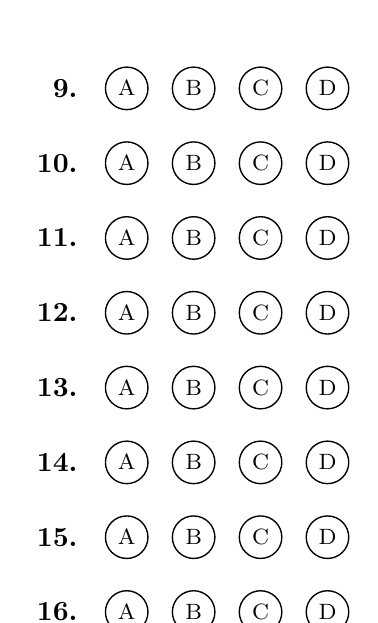
\begin{tikzpicture}[x=1cm,y=1cm]
\node[anchor=east] at (0.55,0.00) {\textbf{9.}};
\draw[line width=0.5pt] (1.05,0.00) circle (0.27);
\node at (1.05,0.00) {\footnotesize A};
\draw[line width=0.5pt] (1.90,0.00) circle (0.27);
\node at (1.90,0.00) {\footnotesize B};
\draw[line width=0.5pt] (2.75,0.00) circle (0.27);
\node at (2.75,0.00) {\footnotesize C};
\draw[line width=0.5pt] (3.60,0.00) circle (0.27);
\node at (3.60,0.00) {\footnotesize D};
\node[anchor=east] at (0.55,-0.95) {\textbf{10.}};
\draw[line width=0.5pt] (1.05,-0.95) circle (0.27);
\node at (1.05,-0.95) {\footnotesize A};
\draw[line width=0.5pt] (1.90,-0.95) circle (0.27);
\node at (1.90,-0.95) {\footnotesize B};
\draw[line width=0.5pt] (2.75,-0.95) circle (0.27);
\node at (2.75,-0.95) {\footnotesize C};
\draw[line width=0.5pt] (3.60,-0.95) circle (0.27);
\node at (3.60,-0.95) {\footnotesize D};
\node[anchor=east] at (0.55,-1.90) {\textbf{11.}};
\draw[line width=0.5pt] (1.05,-1.90) circle (0.27);
\node at (1.05,-1.90) {\footnotesize A};
\draw[line width=0.5pt] (1.90,-1.90) circle (0.27);
\node at (1.90,-1.90) {\footnotesize B};
\draw[line width=0.5pt] (2.75,-1.90) circle (0.27);
\node at (2.75,-1.90) {\footnotesize C};
\draw[line width=0.5pt] (3.60,-1.90) circle (0.27);
\node at (3.60,-1.90) {\footnotesize D};
\node[anchor=east] at (0.55,-2.85) {\textbf{12.}};
\draw[line width=0.5pt] (1.05,-2.85) circle (0.27);
\node at (1.05,-2.85) {\footnotesize A};
\draw[line width=0.5pt] (1.90,-2.85) circle (0.27);
\node at (1.90,-2.85) {\footnotesize B};
\draw[line width=0.5pt] (2.75,-2.85) circle (0.27);
\node at (2.75,-2.85) {\footnotesize C};
\draw[line width=0.5pt] (3.60,-2.85) circle (0.27);
\node at (3.60,-2.85) {\footnotesize D};
\node[anchor=east] at (0.55,-3.80) {\textbf{13.}};
\draw[line width=0.5pt] (1.05,-3.80) circle (0.27);
\node at (1.05,-3.80) {\footnotesize A};
\draw[line width=0.5pt] (1.90,-3.80) circle (0.27);
\node at (1.90,-3.80) {\footnotesize B};
\draw[line width=0.5pt] (2.75,-3.80) circle (0.27);
\node at (2.75,-3.80) {\footnotesize C};
\draw[line width=0.5pt] (3.60,-3.80) circle (0.27);
\node at (3.60,-3.80) {\footnotesize D};
\node[anchor=east] at (0.55,-4.75) {\textbf{14.}};
\draw[line width=0.5pt] (1.05,-4.75) circle (0.27);
\node at (1.05,-4.75) {\footnotesize A};
\draw[line width=0.5pt] (1.90,-4.75) circle (0.27);
\node at (1.90,-4.75) {\footnotesize B};
\draw[line width=0.5pt] (2.75,-4.75) circle (0.27);
\node at (2.75,-4.75) {\footnotesize C};
\draw[line width=0.5pt] (3.60,-4.75) circle (0.27);
\node at (3.60,-4.75) {\footnotesize D};
\node[anchor=east] at (0.55,-5.70) {\textbf{15.}};
\draw[line width=0.5pt] (1.05,-5.70) circle (0.27);
\node at (1.05,-5.70) {\footnotesize A};
\draw[line width=0.5pt] (1.90,-5.70) circle (0.27);
\node at (1.90,-5.70) {\footnotesize B};
\draw[line width=0.5pt] (2.75,-5.70) circle (0.27);
\node at (2.75,-5.70) {\footnotesize C};
\draw[line width=0.5pt] (3.60,-5.70) circle (0.27);
\node at (3.60,-5.70) {\footnotesize D};
\node[anchor=east] at (0.55,-6.65) {\textbf{16.}};
\draw[line width=0.5pt] (1.05,-6.65) circle (0.27);
\node at (1.05,-6.65) {\footnotesize A};
\draw[line width=0.5pt] (1.90,-6.65) circle (0.27);
\node at (1.90,-6.65) {\footnotesize B};
\draw[line width=0.5pt] (2.75,-6.65) circle (0.27);
\node at (2.75,-6.65) {\footnotesize C};
\draw[line width=0.5pt] (3.60,-6.65) circle (0.27);
\node at (3.60,-6.65) {\footnotesize D};
\end{tikzpicture}
\end{minipage}\hfill
\begin{minipage}[t]{0.32\textwidth}\centering
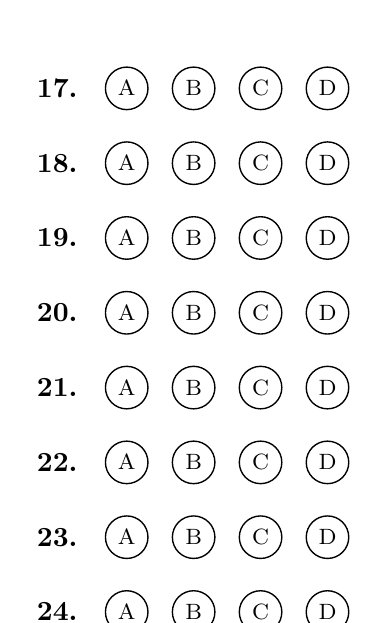
\begin{tikzpicture}[x=1cm,y=1cm]
\node[anchor=east] at (0.55,0.00) {\textbf{17.}};
\draw[line width=0.5pt] (1.05,0.00) circle (0.27);
\node at (1.05,0.00) {\footnotesize A};
\draw[line width=0.5pt] (1.90,0.00) circle (0.27);
\node at (1.90,0.00) {\footnotesize B};
\draw[line width=0.5pt] (2.75,0.00) circle (0.27);
\node at (2.75,0.00) {\footnotesize C};
\draw[line width=0.5pt] (3.60,0.00) circle (0.27);
\node at (3.60,0.00) {\footnotesize D};
\node[anchor=east] at (0.55,-0.95) {\textbf{18.}};
\draw[line width=0.5pt] (1.05,-0.95) circle (0.27);
\node at (1.05,-0.95) {\footnotesize A};
\draw[line width=0.5pt] (1.90,-0.95) circle (0.27);
\node at (1.90,-0.95) {\footnotesize B};
\draw[line width=0.5pt] (2.75,-0.95) circle (0.27);
\node at (2.75,-0.95) {\footnotesize C};
\draw[line width=0.5pt] (3.60,-0.95) circle (0.27);
\node at (3.60,-0.95) {\footnotesize D};
\node[anchor=east] at (0.55,-1.90) {\textbf{19.}};
\draw[line width=0.5pt] (1.05,-1.90) circle (0.27);
\node at (1.05,-1.90) {\footnotesize A};
\draw[line width=0.5pt] (1.90,-1.90) circle (0.27);
\node at (1.90,-1.90) {\footnotesize B};
\draw[line width=0.5pt] (2.75,-1.90) circle (0.27);
\node at (2.75,-1.90) {\footnotesize C};
\draw[line width=0.5pt] (3.60,-1.90) circle (0.27);
\node at (3.60,-1.90) {\footnotesize D};
\node[anchor=east] at (0.55,-2.85) {\textbf{20.}};
\draw[line width=0.5pt] (1.05,-2.85) circle (0.27);
\node at (1.05,-2.85) {\footnotesize A};
\draw[line width=0.5pt] (1.90,-2.85) circle (0.27);
\node at (1.90,-2.85) {\footnotesize B};
\draw[line width=0.5pt] (2.75,-2.85) circle (0.27);
\node at (2.75,-2.85) {\footnotesize C};
\draw[line width=0.5pt] (3.60,-2.85) circle (0.27);
\node at (3.60,-2.85) {\footnotesize D};
\node[anchor=east] at (0.55,-3.80) {\textbf{21.}};
\draw[line width=0.5pt] (1.05,-3.80) circle (0.27);
\node at (1.05,-3.80) {\footnotesize A};
\draw[line width=0.5pt] (1.90,-3.80) circle (0.27);
\node at (1.90,-3.80) {\footnotesize B};
\draw[line width=0.5pt] (2.75,-3.80) circle (0.27);
\node at (2.75,-3.80) {\footnotesize C};
\draw[line width=0.5pt] (3.60,-3.80) circle (0.27);
\node at (3.60,-3.80) {\footnotesize D};
\node[anchor=east] at (0.55,-4.75) {\textbf{22.}};
\draw[line width=0.5pt] (1.05,-4.75) circle (0.27);
\node at (1.05,-4.75) {\footnotesize A};
\draw[line width=0.5pt] (1.90,-4.75) circle (0.27);
\node at (1.90,-4.75) {\footnotesize B};
\draw[line width=0.5pt] (2.75,-4.75) circle (0.27);
\node at (2.75,-4.75) {\footnotesize C};
\draw[line width=0.5pt] (3.60,-4.75) circle (0.27);
\node at (3.60,-4.75) {\footnotesize D};
\node[anchor=east] at (0.55,-5.70) {\textbf{23.}};
\draw[line width=0.5pt] (1.05,-5.70) circle (0.27);
\node at (1.05,-5.70) {\footnotesize A};
\draw[line width=0.5pt] (1.90,-5.70) circle (0.27);
\node at (1.90,-5.70) {\footnotesize B};
\draw[line width=0.5pt] (2.75,-5.70) circle (0.27);
\node at (2.75,-5.70) {\footnotesize C};
\draw[line width=0.5pt] (3.60,-5.70) circle (0.27);
\node at (3.60,-5.70) {\footnotesize D};
\node[anchor=east] at (0.55,-6.65) {\textbf{24.}};
\draw[line width=0.5pt] (1.05,-6.65) circle (0.27);
\node at (1.05,-6.65) {\footnotesize A};
\draw[line width=0.5pt] (1.90,-6.65) circle (0.27);
\node at (1.90,-6.65) {\footnotesize B};
\draw[line width=0.5pt] (2.75,-6.65) circle (0.27);
\node at (2.75,-6.65) {\footnotesize C};
\draw[line width=0.5pt] (3.60,-6.65) circle (0.27);
\node at (3.60,-6.65) {\footnotesize D};
\end{tikzpicture}
\end{minipage}\hfill

\vspace{3em}
\begin{center}
\large Score \quad \underline{\hspace{2cm}} \,/\, 24
\end{center}


\newpage
\begin{center}
  {\Large\bfseries Formula Sheet}\\[3pt]
  {\small\itshape Use this page only if your exam provides a formula sheet.}\\[2pt]
  \rule{\textwidth}{0.4pt}
\end{center}

\subsection*{Fitness}
\begin{center}\renewcommand{\arraystretch}{2.1}
\begin{tabular}{r@{\;}l@{\qquad}l}
  \(w\) & \(=\ \text{viability} \times \text{fecundity}\) & absolute fitness, offspring left per zygote\\
  \(W\) & \(=\ w / w_{\max}\) & relative fitness\\
  \(s\) & \(=\ 1 - W\) & selection coefficient
\end{tabular}\end{center}

\subsection*{Mean fitness and the general equation}
\begin{align*}
  \overline{W} &= f(AA)\,W_{AA} + f(Aa)\,W_{Aa} + f(aa)\,W_{aa}\\[4pt]
  q' &= \frac{\tfrac{1}{2}\,f(Aa)\,W_{Aa} + f(aa)\,W_{aa}}{\overline{W}}, \qquad \Delta q = q' - q
\end{align*}
Under Hardy--Weinberg, \(f(AA)=p^2\), \(f(Aa)=2pq\), \(f(aa)=q^2\). With counted individuals that selection acts on directly, use the counted frequencies.

\subsection*{Average excess}
\begin{align*}
  \alpha_a &= q\,W_{aa} + p\,W_{Aa} - \overline{W}, & \Delta q &= \frac{q}{\overline{W}}\,\alpha_a\\[4pt]
  \alpha_A &= p\,W_{AA} + q\,W_{Aa} - \overline{W}, & \Delta p &= \frac{p}{\overline{W}}\,\alpha_A
\end{align*}
Requires Hardy--Weinberg genotype frequencies.

\subsection*{Special models (\(q\) is always the allele selected against)}
\begin{align*}
  \text{Against the recessive:}\quad \Delta q &= \frac{-s\,p\,q^2}{1 - s\,q^2}\\[4pt]
  \text{Against the dominant:}\quad \Delta q &= \frac{-s\,p^2 q}{1 - 2sq + sq^2}
\end{align*}

\subsection*{Heterozygote advantage or disadvantage}
\[
  \hat{q} = \frac{s_1}{s_1 + s_2}
\]
with \(s_1\) for the \(p\) homozygote and \(s_2\) for the \(q\) homozygote. The equilibrium is stable under heterozygote advantage and unstable under heterozygote disadvantage.

\label{LastPage}
\end{document}